\chapter{Módulo Driver INDI}


En esta parte del proyecto nos centraremos en exponer como se ha creado el driver INDI específico para el dispositivo desarrollado bajo la tecnología Arduino en los capítulos anteriores de este mismo proyecto.

Este driver dotará a este dispositivo de la funcionalidad necesaria para poder funcionar en remoto, bajo el protocolo de control INDI, destinado a dispositivos astronómicos. 

Para ello se trabajará con la versión implementada en Java de este protocolo, \textbf{INDI for Java} \cite{INDIFJ}, por lo cual el lenguaje de programación que usaremos es Java.


\section{Breve introducción a INDI}

INDI consiste a su nivel más básico en un protocolo que permite el control, automatización, obtención de datos e intercambio de los mismos entre distintos dispositivos hardware y programas cliente. 

La idea subyacente en el protocolo INDI es desacoplar aspectos específicos del hardware, haciendo que cambios en el hardware no impliquen necesariamente cambios en el software.

\begin{figure}[h]
	\begin{center}
		
\includegraphics[width=0.5\textwidth]{../images/indi.png}
		\caption[INDI Logo]{Logo de INDI  Fuente: \cite{indi}}
		\label{fig:indi}
	\end{center}
\end{figure}

Para conseguir un desacople efectivo entre los clientes y el hardware se define un protocolo basado en \textbf{XML} que permite abstraer los dispositivos hardware como conjuntos de \textbf{propiedades} que pueden ser leídas, y modificadas por los clientes (siempre estableciendo las restricciones oportunas).


\subsection{Drivers, Servidores y Clientes INDI}

Pese a que nivel más básico INDI es ``simplemente'' una especificación de un protocolo basado en XML, a un nivel superior se distinguen tres entidades diferentes que interaccionan entre sí para tener un sistema de control plenamente funcional (figuras~\ref{fig:DriverServerIndi} y \ref{fig:indi-tophology}):


\begin{itemize}
	\item \textbf{Drivers:} Son programas que se ejecutarán (normalmente) en la máquina donde se conectan los dispositivos hardware. Son los encargados de la comunicación directa con los dispositivos y su abstracción a propiedades INDI.
		
	\item \textbf{Servidor:} Es un programa cuya función principal es ejecutar los drivers y permitir la conexión a los mismos por parte de los clientes (funciona de un modo similar a un proxy). Normalmente reside en la máquina donde están conectados los dispositivos, aunque en principio se pueden crear estructuras de red tipo árbol de servidores. El intercambio de información entre el servidor y los drivers se realiza utilizando el protocolo INDI.
	
	\item \textbf{Cliente:} Es un programa que permite conectar con uno o más servidores y su función principal e hacer de \textbf{interfaz} con el usuario. Para ello conecta (usualmente a través de la red) con el servidor e intercambia información sobre los dispositivos utilizando el protocolo INDI. Es interesante recalcar que los clientes pueden ser de cualquier estilo: desde programas con interfaz de usuario avanzadas, hasta programas simples en línea de comandos scripts completamente automáticos que controlen o monitoricen los dispositivos.
\end{itemize}


\begin{figure}[h]
	\centering
	\includegraphics[width=1\linewidth]{../images/INDIPipeline}
	\caption[Pipeline INDI]{\textbf{Pipeline INDI}, flujo de información y conversión en diferentes entidades. (String Comando Serie - Propiedad Indi - Documento XML )}
	\label{fig:DriverServerIndi}
\end{figure}

\begin{figure}
	\centering
	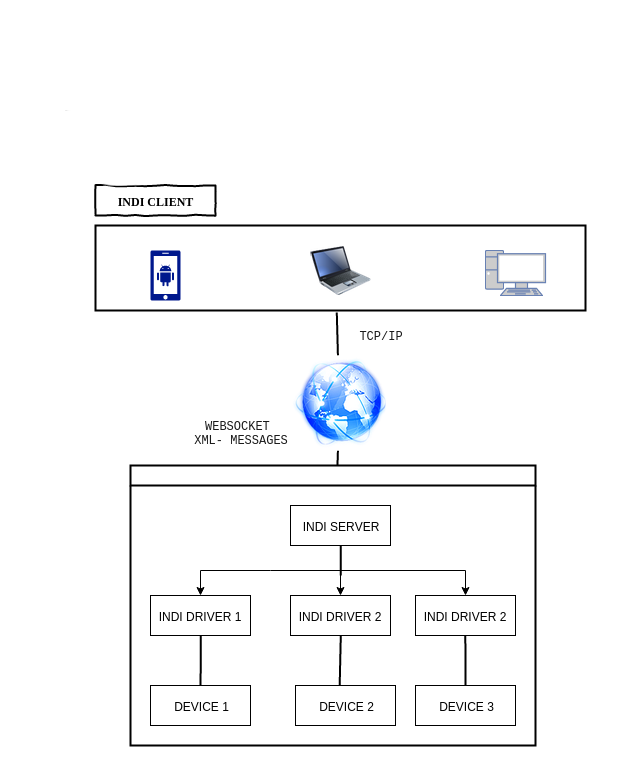
\includegraphics[width=1\linewidth]{../images/indi-tophology}
	\caption[Arquitectura Servidor - Driver INDI]{Arquitectura Servidor - Driver INDI}
	\label{fig:indi-tophology}
\end{figure}


La biblioteca \textbf{INDI} original está escrita en lenguaje \textbf{C}, pero existe una implementación completa realizada en \textbf{Java} y que se encuentra en constante mejora. En la página oficial de \href{http://indilib.org/develop/indiforjava.html}{INDI} podemos encontrar toda la información sobre nuevas versiones y la documentación para poder utilizarla. La principal ventaja de poder usar \textbf{Java} es que podemos implementar drivers y clientes con la potencia de un lenguaje orientado a objetos y combinarlo con otras tecnologías como los dispositivos móviles basados en la plataforma \textbf{Android}  \href{https://play.google.com/store/apps/details?id=com.jtbenavente.jaime.indiandroidui&hl=es}{(\textbf{enlace descarga de Remote Observatory (App Android)})} 





\subsection{Propiedades INDI}

El protocolo INDI define un conjunto de 5 propiedades que envían los diferentes drivers para formar la interfaz del cliente. Las propiedades se relacionan con el tipo de dato que maneja el dispositivo para controlar una característica concreta:

\begin{itemize}
	\item \textbf{Textos:} Son cadenas de caracteres ordenados arbitrariamente.
	
	\item \textbf{Números:} Son cantidades numéricas. Además de la cantidad numérica se envían otros parámetros que sirven para el formato de su visualización y configuración (mínimo, máximo, paso, etc.).
	
	\item \textbf{Switches:} Son propiedades binarias con estado encendido o apagado. Sus agrupaciones pueden ser de tres tipos diferentes:
	
	\begin{itemize}
		\item \textbf{Una de muchas:} para todas las opciones se tiene que seleccionar
		obligatoriamente una.
		
		\item \textbf{Como máximo una:} de todas las opciones se puede seleccionar
		como máximo una.
		
		\item \textbf{Cualquiera de muchas:} se podrán seleccionar todas las que se
		deseen.
		
	\end{itemize}	
	
	\item \textbf{Lights:} Son propiedades de solo lectura, que pueden estar en cada uno de los cuatro
	estados que se definen.
	
	\begin{itemize}
		\item \textbf{Inactivo:} Luz de color gris.
		\item \textbf{Alerta:} Luz de color rojo.
		\item \textbf{Ocupado:} Luz de color amarillo.
		\item \textbf{Ok:} Luz de color verde.
	\end{itemize}
		
	\item \textbf{BLOBs:} Datos binarios cualesquiera.
\end{itemize}


\section{Diseño del Driver INDI}

A continuación se desglosa información sobre el proceso de diseño y planificación de este módulo.

\subsection{Requisitos funcionales}

\begin{itemize}
	\item \textbf{RF-1.}: Crear conexión con dispositivo enfocador Ardufocuser.
	\item \textbf{RF-2.}: Controlar posición del enfocador Ardufocuser, permitir moverlo a la posición deseada.
	\item \textbf{RF-3.}: Modificar velocidad del enfocador.
	\item \textbf{RF-4.}: Modificar pasos por pulso que se mueve.
	\item \textbf{RF-5.}: Modificar posición relativa del enfocador.
	\item \textbf{RF-5.}: Mostrar temperatura del enfocador.
	\item \textbf{RF-5.}: Establece límite software del enfocador.
	\item \textbf{RF-6.}: Mostrar aviso si se alcanza un límite software.
	\item \textbf{RF-7.}: Mostrar aviso si se alcanza un límite hardware.
	\item \textbf{RF-8.}: Encender y apagar la iluminación de la pantalla lcd.		
\end{itemize}

\subsection{Requisitos no funcionales}
\begin{itemize}
	\item \textbf{RNF-1.}: El intercambio de mensajes por el puerto serie tiene que ser eficiente y tolerante a perdida de mensajes.
	\item \textbf{RNF-2.}: La información ha de presentarse al usuario de una forma clara e intuitiva.
	\item \textbf{RNF-3.}: Debe ser compatible con los clientes INDI que existen actualmente.
\end{itemize}

\subsection{Arquitectura INDI for Java}

Debemos conocer la estructura que tiene un Driver INDI. Para ello se recurrimos a la referencia oficial   \href{http://www.indilib.org/develop/indiforjava/i4j-indi-driver.html}{indiforjava}, donde podemos encontrar una buena guía para implementar un Driver, junto un ejemplo simple. 

\textbf{INDI for Java}, ya cuenta con una clase abstracta que define muchos de los atributos y métodos mínimos con los que debe contar un enfocador ``\texttt{Focuser}'' genérico. Debemos heredar de dicha clase para definir nuestro \texttt{ArduFocuserDriver} particular, añadiendo nuevos atributos e implementando los métodos abstractos existentes. 


\begin{figure}
\centering
\includegraphics[width=1\linewidth]{../images/indi_classes}
\caption{Diagrama de clases Driver INDI}
\label{fig:indi_classes}
\end{figure}



\paragraph{Propiedades a implementar}

Para ello lo primero que tenemos que hacer es definir exactamente las propiedades que tiene nuestro dispositivo, el tipo y si son lectura, escritura o ambas. 

Dichas propiedades (tabla~\ref{fig:propiedades_indi}) serán comunicadas al cliente INDI para que este puede hacer una representación en la interfaz gráfica.

\begin{table}[h]
	\centering

	\begin{tabular}{|l|l|l|l|l|}
		\hline
		Descripción                        & RW/OW/OR  & Tipo Propiedad &          \begin{tabular}[c]{@{}l@{}}   
			                                                                          Mininimo \\ 
			                                                                          Máximo   \\ 
			                                                                          Step     \\
			                                                                     \end{tabular} \\ \hline\hline
			                                                                     
			                                                                     
		Posición Actual                    & RW        & Number&            \begin{tabular}[c]{@{}l@{}}
																						MinimumAbsPos       \\
																						MaximumAbsPos    \\
																						1 \\
																		        \end{tabular} \\ \hline
																				    
		Velocidad                          & RW        & Number&             \begin{tabular}[c]{@{}l@{}}
			                                                                         1              \\
			                                                                         MaximumSpeed	\\
			                                                                         1			    \\
			                                                                    \end{tabular} \\ \hline
			                                                                    
		Movimiento enfocador           & OR       & SwitchOneOrNone&    --           \\ \hline
		Pasos por pulso                    & RW       & Number&            \begin{tabular}[c]{@{}l@{}}
																					1  \\
																					99 \\
																					1  \\ 
																			   \end{tabular} \\ \hline

		Temperatura                        & OR       & Number&             --\\ \hline
		Límite Hardware                     & OR       & Switch&             --\\ \hline
		Límite Software                     & OR       & Switch&             --\\ \hline	
		Posición Relativa                  & RW       & Number&            \begin{tabular}[c]{@{}l@{}}
																					MinimumAbsPos  \\
																					MaximumAbsPos \\
																					1  \\ 
																				\end{tabular} \\ \hline	
		Iluminación LCD                       & RW       & Switch&             --\\  \hline
	                  
	\end{tabular}
		\caption{Propiedades del Driver INDI del Ardufocuser}
	\label{fig:propiedades_indi}
\end{table}


\section{Implementación}


\paragraph{Gestionar conexión serie}

La comunicación directa con \textbf{Ardufocuser} se basa en el protocolo serie. Por tanto el primer paso es hacer que nuestra rutina Java se conecte al puerto serie de Arduino. Para ello se hace uso de la biblioteca \textbf{RXTX library}, junto con un conector específico para Arduino, \textbf{JavaDuino} \cite{JavaDuino}. En el fragmento de código~\ref{lst:ejemplo_libreria_serial_commandd} podemos ver un ejemplo de su uso.


\begin{lstlisting}[language=javascript, caption={Ejemplo biblioteca \texttt{SerialCommand}},label={lst:ejemplo_libreria_serial_commandd}]
 import gnu.io.SerialPortEvent;
 import gnu.io.SerialPortEventListener;
 public class Main {
 
	 public static void main(String[] args) { 
		 // Abrir la conexión Arduino.
		 ArduinoConnection ac = new ArduinoConnection();
		 boolean connected = ac.connectToBoard();
		 
		 if (connected) {
			 System.out.println("Conectado!");
		 } else {
			 System.out.println("No se puede conectar con Arduino :-(");
			 return;
		 }
		 
		 // Añadimos escuchador, que responde a un evento série.
		 ac.addListener(new SampleListener(ac));
		 // Enviar mensajes por puerto serie.
		 ac.sendString("Arduino!");
		 // Cerrar la conexión.
		 ac.close();
	 }
	 
	 private static class SampleListener implements SerialPortEventListener {	 
		 private ArduinoConnection ac;	 
			 public SampleListener(ArduinoConnection ac) {
			 this.ac = ac;
		 }
		 		 
		 @Override
		 public void serialEvent(SerialPortEvent serialPortEvent) {
			 // Callback que se ejecuta con un evento serie.
			 if (serialPortEvent.getEventType() == SerialPortEvent.DATA_AVAILABLE) {
				 String inLine = ac.readLine();
				 System.out.println("GOT: " + inLine);
			 }
		 }
	 }
 }
\end{lstlisting}


\texttt{ArduinoConnection} cuenta con los siguiente métodos:

\begin{itemize}
	\item \texttt{ArduinoConnection()} : Constructor principal.
	\item \texttt{connectToBoard()} : Se conecta a la placa Arduino.
	\item \texttt{addListener(SerialPortEventListener)} : Añade un escuchador, permite ejecutar una función callback dado un evento serie, sin bloquear el flujo de la rutina main.
	\item \texttt{sendString(String)} : Envía una cadena e texto a Arduino.
\end{itemize}

Otro aspecto importante en la implementación del driver INDI es la creación e inicialización de las propiedades que hemos comentado.

Para ello se debe crear una instancia \texttt{INDIProperty}, que es el objeto que representa a la propiedad en concreto, indicando el grupo de propiedades al que pertenece, el estado inicial así como si es de lectura, escritura o lectura escritura.

Una propiedad puede tener varios elementos: de manera informal podemos decir que los elementos son las diferente variables que componen una propiedad. Cuando instanciamos un elemento debemos pasar como parámetro la propiedad a la que pertenece. En el fragmento de códgo~\ref{lst:ejemplo_iniciar_propiedad_indi} podemos ver un ejemplo de inicialización de una propiedad. Entre otras se muestra la propiedad definida en el ejemplo anterior.





\begin{lstlisting}[language=javascript, caption={Ejemplo iniciar una propieda INDI Numérica},label={lst:ejemplo_iniciar_propiedad_indi}]
// Propiedad numérica para informar de la temperatura.
private INDINumberProperty temperatureP;

// Elemento numérico para informar de la temperatura.
private INDINumberElement temperatureE;

// Inicializador propiedad para manejar temperatura.
private void inizializeTempretureProperty() {
	if (temperatureP == null) {
		// Se crea la propiedad, con el estado inicial, indicando el conjunto al que pertenece y si es escritura/lectura.
		temperatureP = new INDINumberProperty(this, "temperature", "Temperature", "Control", PropertyStates.IDLE, PropertyPermissions.RO);
		temperatureE = temperatureP.getElement("temperature_value");
		if (temperatureE == null) {
			// La propiedad 
			temperatureE = new INDINumberElement(temperatureP, "temperature", "Temperature", "1", "1", "99", "1", "%f");
		}
	}
}
\end{lstlisting}










\section{Instalación servidor}

Para llevar a cabo todas las pruebas necesarias durante el desarrollo el servidor INDI se ha instalado en un mini-pc Raspberry-Pi, haciendo uso de la distribución Raspbian. El propósito de esta máquina es doble, su uso principal como \textbf{servidor astronómico INDI} (figura~\ref{fig:raspberry}) y además al contar con todo el entorno de Arduino, facilita la tarea de \textbf{actualización del firmware}. En la figura~\ref{fig:diagramaGeneral} encontramos un diagrama completo del sistema Ardufocuser contando con el servidor INDI en la Raspberry Pi.

\begin{figure}[h]
\centering
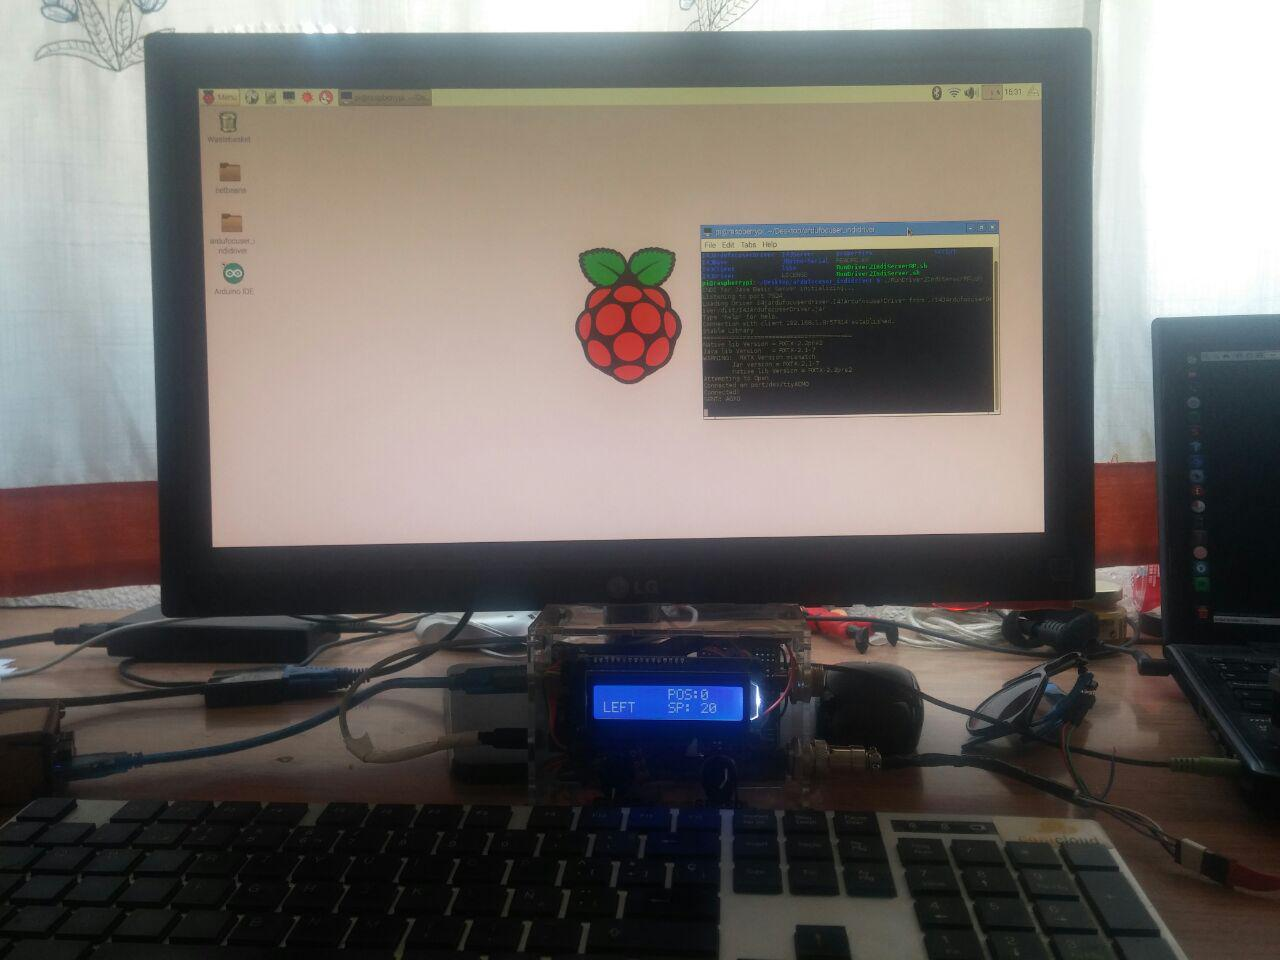
\includegraphics[width=1\linewidth]{../images/rasp_server}
\caption[Servidor INDI funcionando en Raspberry Pi]{Servidor INDI funcionando en Raspberry Pi}
\label{fig:raspberry}
\end{figure}

\begin{figure}
\centering
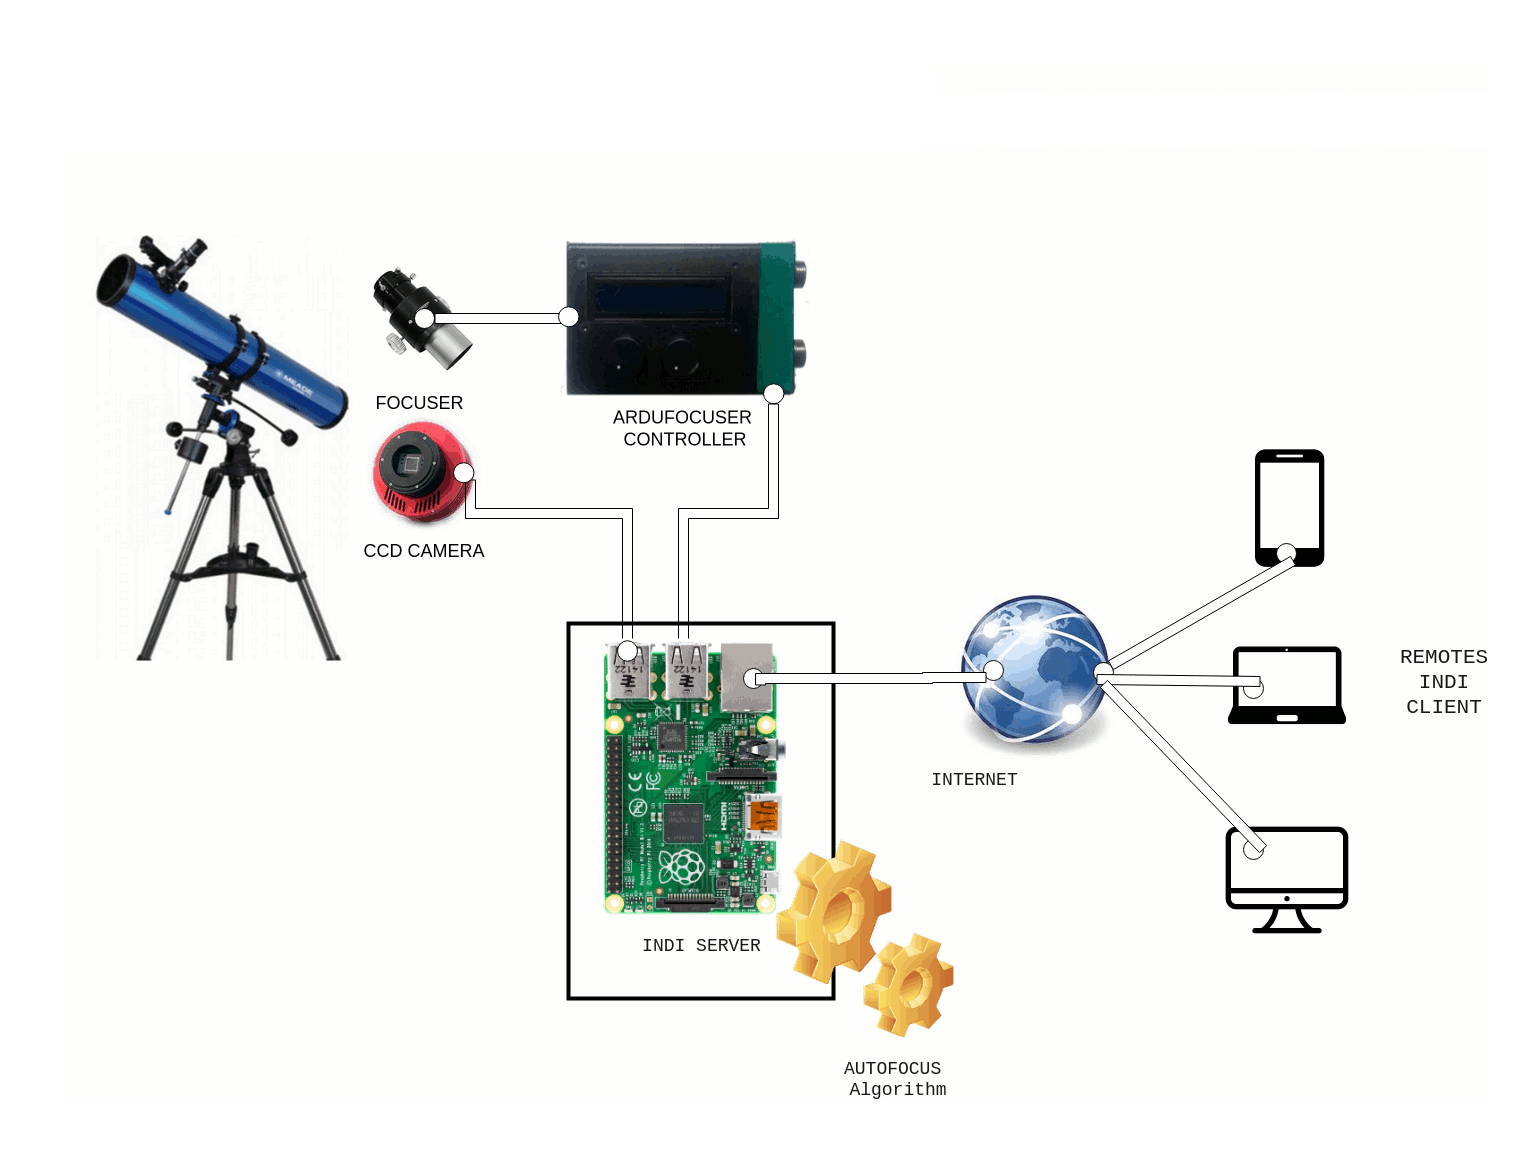
\includegraphics[width=1\linewidth]{../images/diagramaGeneral}
\caption[Diagrama completo del sistema Ardufocuser]{Diagrama completo del sistema Ardufocuser}
\label{fig:diagramaGeneral}
\end{figure}


Para ello se han instalado las siguientes herramientas:
\begin{itemize}
	\item \textbf{Java}, entorno de ejecución Java.
	\item \textbf{Netbeans} Entorno de desarrollo Java.
	\item \textbf{Arduino IDE}, permite cargar el firmware en la placa.
	\item \textbf{KStars}, cliente INDI.
	\item \textbf{Servidor INDI + Driver INDI}.
\end{itemize}

La biblioteca necesaria para que Raspberry y Arduino se puedan comunicar mediante puerto serie es \textbf{RXTX} en su versión para Java. 

\begin{center}
\texttt{> sudo apt-get install librxtx-java}
\end{center}

En los fragmentos de código~\ref{lst:script_inicio_indi} y \ref{lst:script_inicio_2} se muestran los scripts que se han creado / modificado en la distribución Raspbian para ejecutar automáticamente el servidor INDI.

\begin{lstlisting}[language=bash, caption={Script de inicio del servidor INDI},label={lst:script_inicio_indi}][h!]
#! /bin/sh
# /etc/init.d/indiserver-init

### BEGIN INIT INFO
# Provides: 		indiserver-init
# Required-Start: 	$all
# Required-Stop:	$remote_fs $syslog
# Default-Start:	2 3 4 5
# Default-Stop:		0 1 6
# Short-Description:	Run Indi Server.
# Description:		Run Indi Server with Driver for Ardufocuser.
### END INIT INFO

case "$1" in
start)
echo "IndiServer Runing"
/home/pi/Desktop/ardufocuser_indidriver/RunDriver2IndiServerRPBeep.sh
;;
stop)
echo "IndiServer Stoping"
;;
*)
echo "Modo de uso: /etc/init.d/indiserver-init {start|stop}"
exit 1
;;
esac

exit 0
\end{lstlisting}


\begin{lstlisting}[language=bash, caption={Script de inicio del servidor INDI (2)},label={lst:script_inicio_2}]
#!/bin/bash

# Emite un beep por un zumbador.
python /home/pi/Desktop/ardufocuser_indidriver/beepOK.py

# Ejecuta Servidor INDI con el correspondiente Driver como módulo.
java  -Djava.library.path=/usr/lib/jni -cp /usr/share/java/RXTXcomm.jar  -jar /home/pi/Desktop/ardufocuser_indidriver/I4JServer/dist/I4JServer.jar -add=/home/pi/Desktop/ardufocuser_indidriver/I4JArdufocuserDriver/dist/I4JArdufocuserDriver.jar
\end{lstlisting}





\subsection{Crear imagen Rasbindi}

Para facilitar la instalación del sistema en la Raspberry se ha creado una imagen de todo el entorno. La imagen la podemos descargar directamente del siguiente enlace:


\href{https://drive.google.com/open?id=0Bz7iXJ4BvZ9SbnJPZWkweVhUVjQ}{Enlace para desscargar \textbf{Raspbindi}, imagen personalizada con un servidor INDI configurado.}






\section{Pruebas}

Para este módulo se han realizado pruebas de caja negra, es decir, sin conocer detalles internos del dispositivo tratamos de reproducir posibles casos de uso, y se comprueba si las salidas corresponden con lo esperado. 


Para las pruebas se han usado dos clientes INDI diferentes, anteriormente comentados, KStars (Linux)~\ref{fig:kstar_driver1} y  Observatorio Remoto (Android)~\ref{fig:remote_obs}.


\begin{figure}
	\centering
	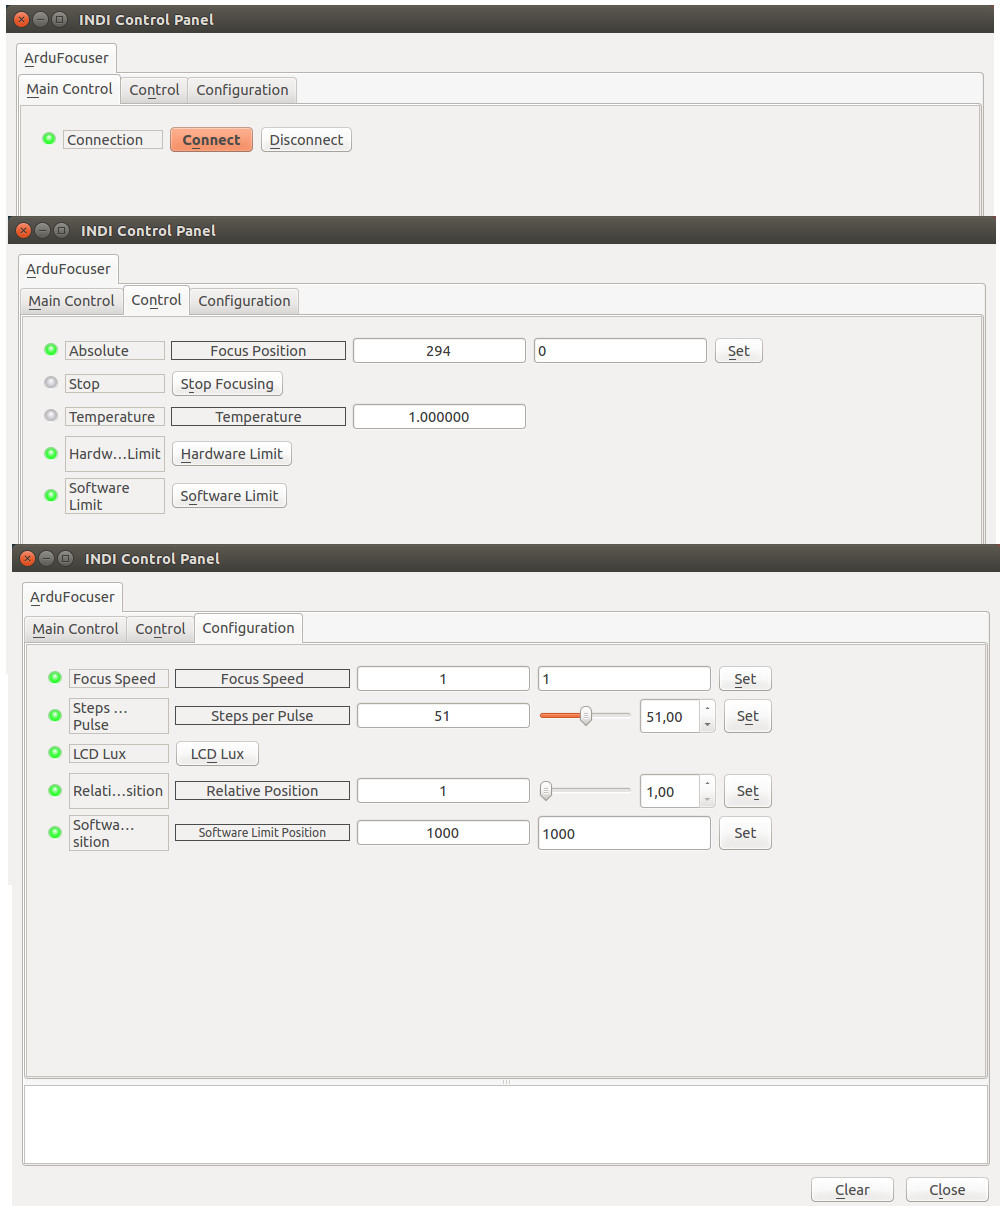
\includegraphics[width=0.8\linewidth]{../images/kstar_driver_full}
	\caption[Pruebas desde KStars]{Se realizan pruebas desde KStars (Cliente de Escritorio)}
	\label{fig:kstar_driver1}
\end{figure}

 \begin{figure}[h]
	\centering
	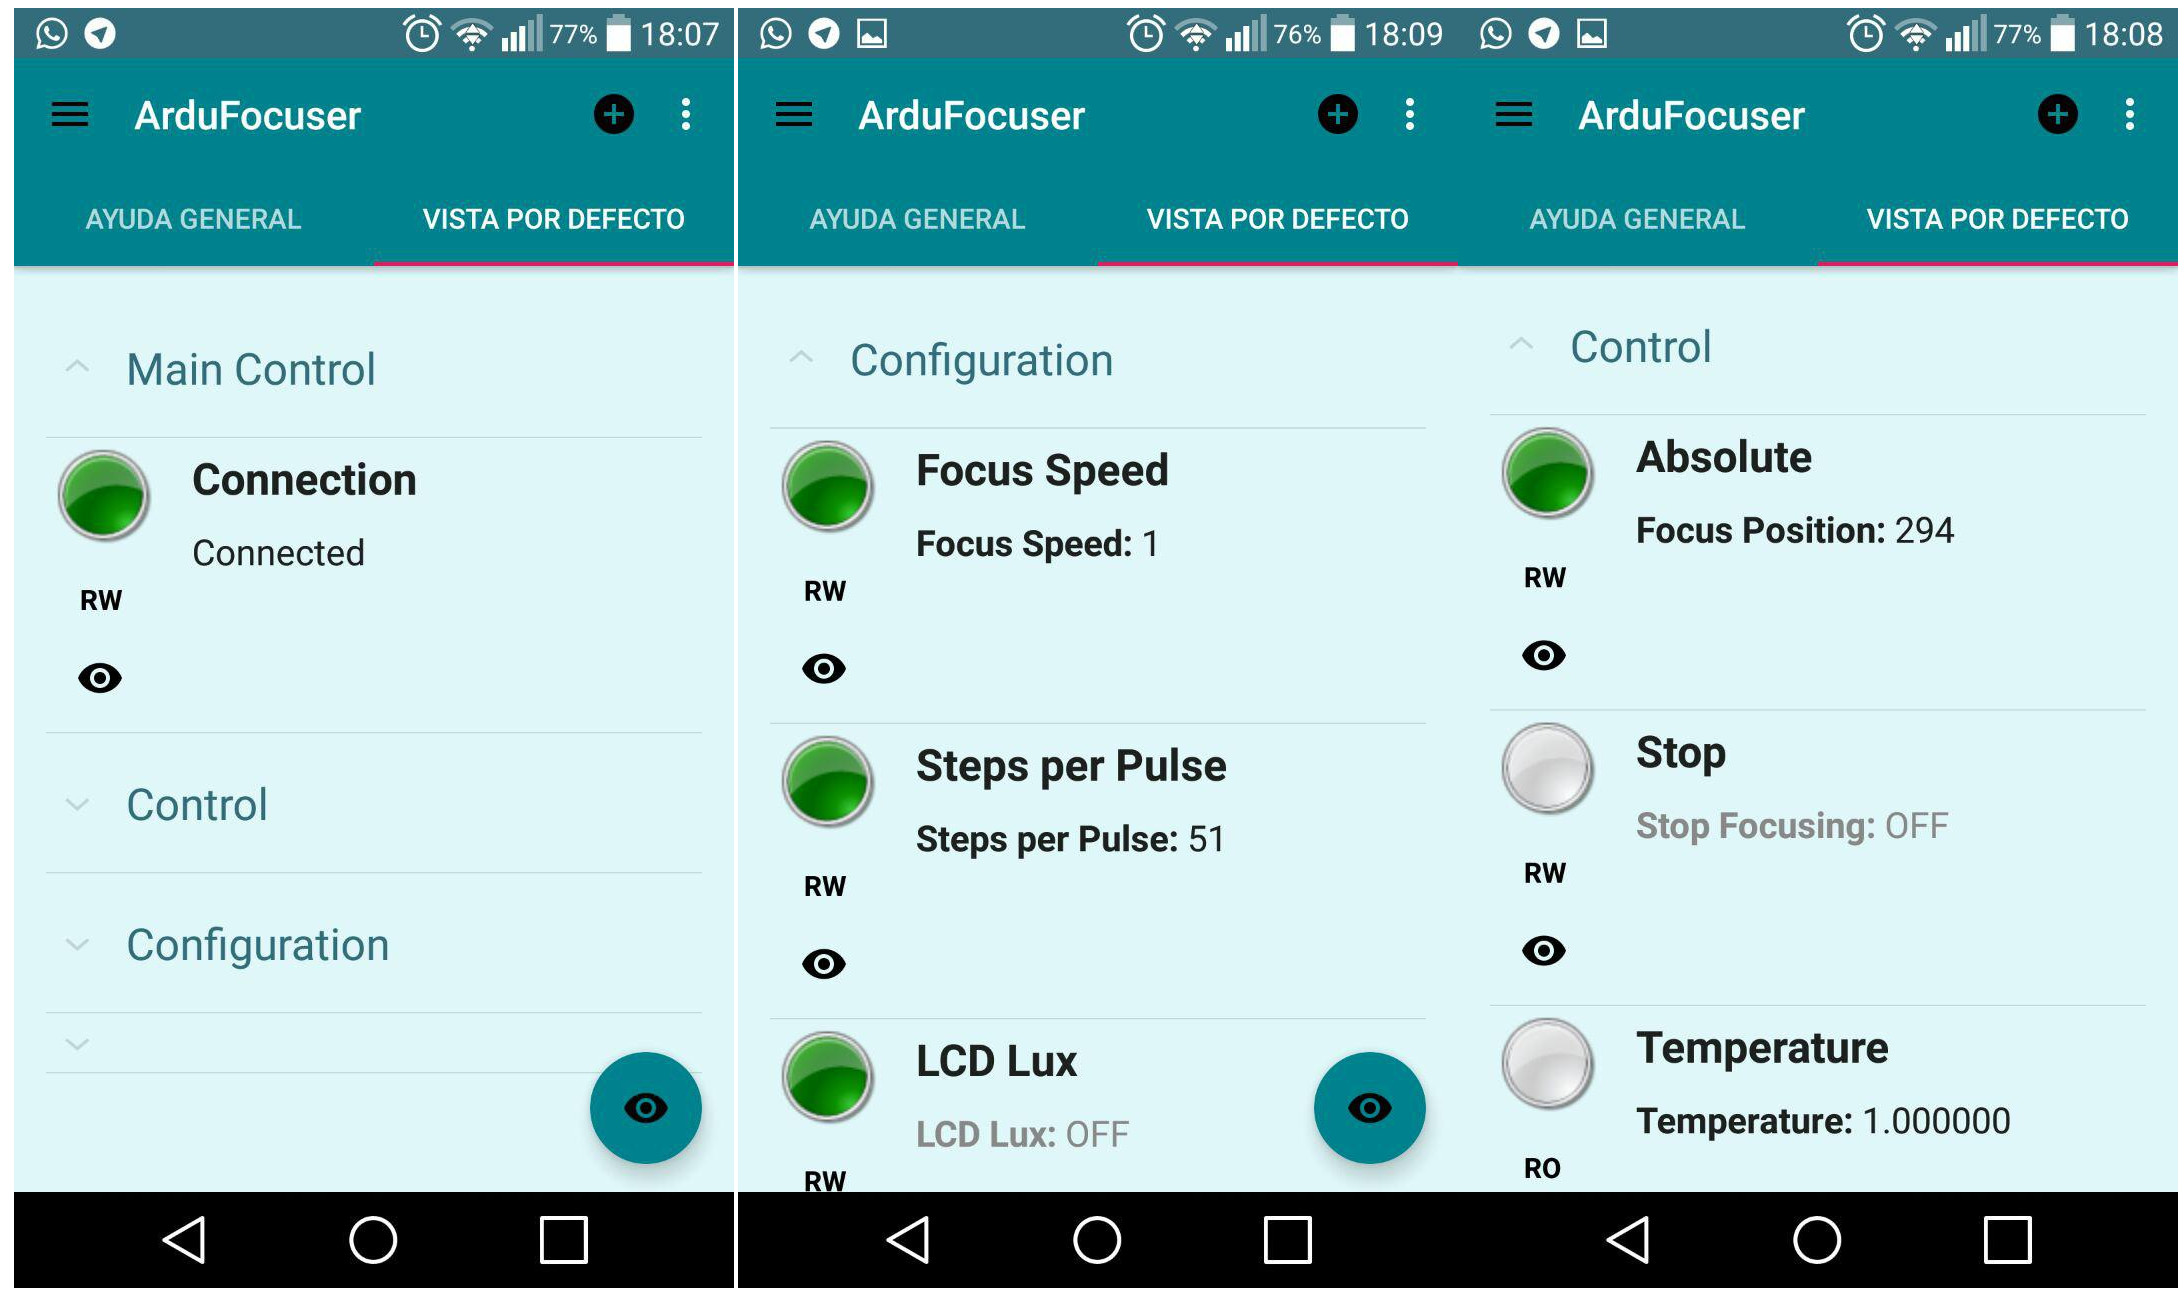
\includegraphics[width=1\linewidth]{../images/obs_remoto_driver_full}
	\caption[Pruebas desde Observatorio Remoto]{Se realizan pruebas desde Observatorio Remoto (Cliente Android)}
	\label{fig:remote_obs}
\end{figure}

En las tablas~\ref{tab:cas1}, \ref{tab:cas2}, \ref{tab:cas3} y \ref{tab:cas4} se pueden ver ejemplos de dichos casos de prueba. Además, en las figuras~\ref{fig:test_1} y \ref{fig:test_2} podemos ver los resultados visuales de la prueba de conexión (con el cliente kstars) al driver y encendido del mismo.

\begin{table}[h]
	\centering

	\begin{tabular}{|l|l|}
		\hline
		ID caso de prueba             &  1 \\ \hline
		Nombre prueba                 &  Conectar a servidor INDI con driver Ardufocuser \\ \hline
		Autor de la prueba            &  José Miguel López \\ \hline
		Responsable diseño            &  José Miguel López \\ \hline
		Pasos y condiciones ejecución &  \begin{tabular}[c]{@{}l@{}}
			- Ejecutar cliente INDI. \\
			- Ir a Device Manager en KStars y pulsar en Add. \\
			- Introducir IP y puerto del servidor INDI. \\
			- Pulsar botón Connect. \\
		\end{tabular} \\ \hline
		Resultado deseado             & \begin{tabular}[c]{@{}l@{}}
			Debe aparecer una nueva ventana \\
			donde se muestran las propiedades \\
			y dispositivos INDI, organizados en pestañas.\\
			
		\end{tabular} \\ \hline
		
		Resultado obtenido            &  \begin{tabular}[c]{@{}l@{}}
			Aparece una nueva ventana \\
			donde se muestran las propiedades\\ de los dispositivos INDI.\\
		\end{tabular} \\ \hline
		Estado caso de prueba         &  Éxito\\ \hline
		Errores asociados             &  Ninguno\\ \hline
		Comentario                    &  \\ \hline
	\end{tabular}
		\caption{Caso de prueba, conectar con servidor INDI}
	\label{tab:cas1}
\end{table} 


\begin{figure}
	\centering
	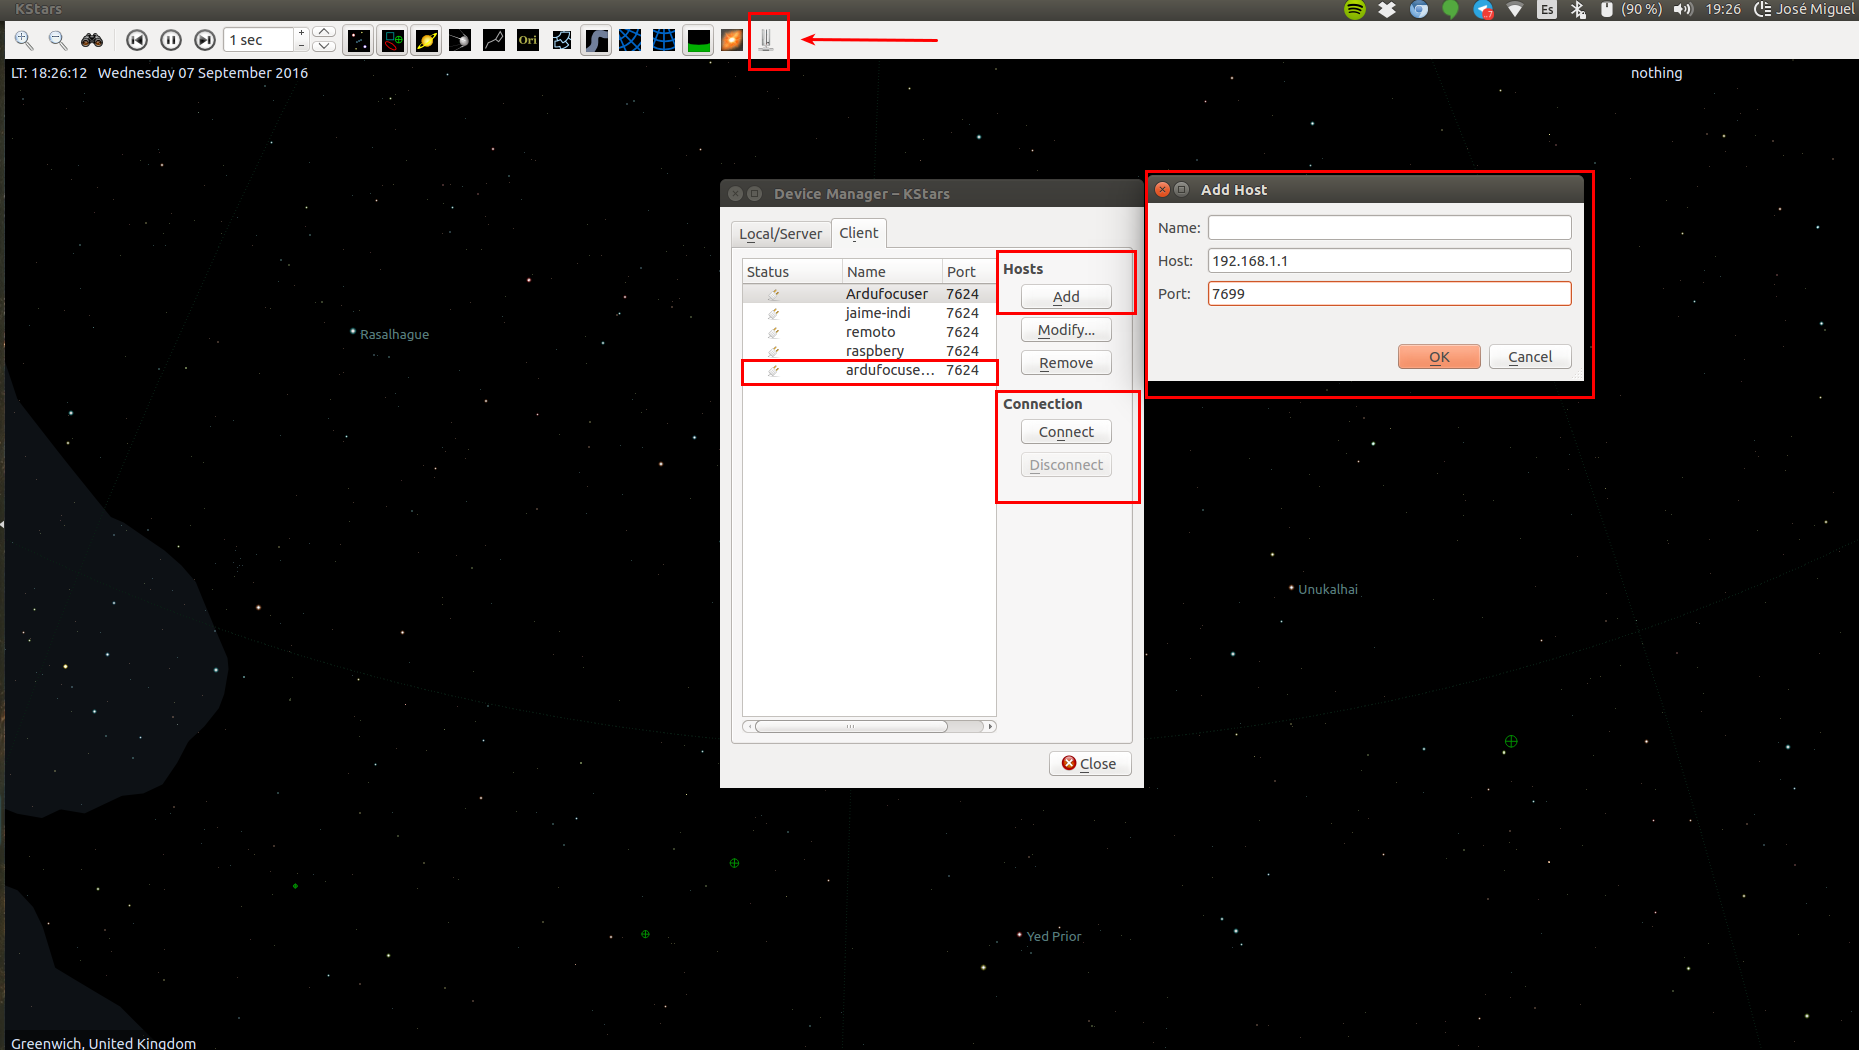
\includegraphics[width=1\linewidth]{../images/test_1}
	\caption{Conectando el servidor INDI con el driver Ardufocuser}
	\label{fig:test_1}
\end{figure}

 

\begin{table}[h]
	\centering

	\begin{tabular}{|l|l|}
		\hline
		ID caso de prueba             &  2 \\ \hline
		Nombre prueba                 &  Conectar Ardufocuser \\ \hline
		Autor de la prueba            &  José Miguel López \\ \hline
		Responsable diseño            &  José Miguel López \\ \hline
		Pasos y condiciones ejecución &  \begin{tabular}[c]{@{}l@{}}
			- Partimos del resultado obtenido \\
			en el caso de uso anterior.\\
			- Ir a la pestaña \texttt{Ardufocuser}\\
			- Ir a la pestaña \texttt{Main Control}\\
			- Pulsar \texttt{Connect}
		\end{tabular} \\ \hline
		Resultado deseado             & \begin{tabular}[c]{@{}l@{}}
			Debe cambiar la luz de la propiedad a verde. \\
			Se activan dos pestañas adicionales\\\texttt{Control} y \texttt{Configuration}. \\
		\end{tabular} \\ \hline
		
		Resultado obtenido            &  \begin{tabular}[c]{@{}l@{}}
			Cambiar la luz de la propiedad a verde. \\
			Se activan dos pestañas adicionales\\\texttt{Control} y \texttt{Configuration}. \\
		\end{tabular} \\ \hline
		Estado caso de prueba         &  Éxito\\ \hline
		Errores asociados             &  Ninguno\\ \hline
		Comentario                    &  \\ \hline
	\end{tabular}
		\caption{Caso de prueba, conectar Ardufocuser}
	\label{tab:cas2}
\end{table} 


\begin{figure}
	\centering
	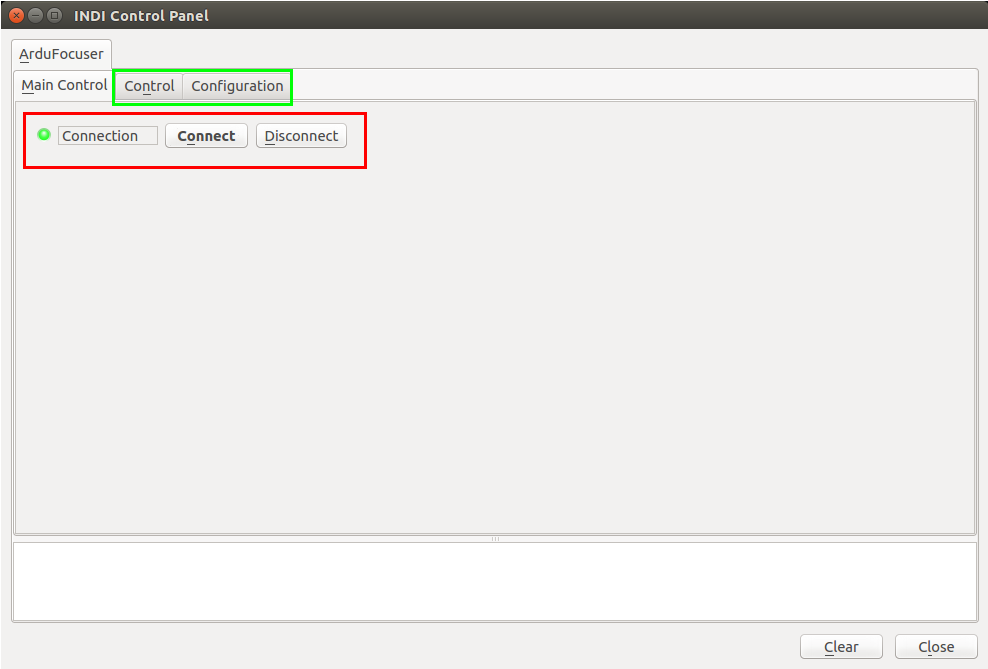
\includegraphics[width=1\linewidth]{../images/01_connection}
	\caption{Conectando el Ardufocuser a través de Kstars}
	\label{fig:test_2}
\end{figure}


\begin{table}[h]
	\centering

	\begin{tabular}{|l|l|}
		\hline
		ID caso de prueba             &  3 \\ \hline
		Nombre prueba                 &  Modificar velocidad del motor \\ \hline
		Autor de la prueba            &  José Miguel López \\ \hline
		Responsable diseño            &  José Miguel López \\ \hline
		Pasos y condiciones ejecución &  \begin{tabular}[c]{@{}l@{}}
			- Partimos del resultado obtenido \\
			en el caso de uso anterior.\\
			- Ir a la pestaña \texttt{Ardufocuser}.\\
			- Ir a la pestaña \texttt{Configuration}.\\
			- Modificar valor \texttt{Focus Speed} y pulsar en \texttt{Set}.
		\end{tabular} \\ \hline
		Resultado deseado             & \begin{tabular}[c]{@{}l@{}}
		    Debe cambiar la luz de la propiedad a verde. \\
		    Debe cambiar el valor SP en la pantalla LCD \\
		\end{tabular} \\ \hline
		
		Resultado obtenido            &  \begin{tabular}[c]{@{}l@{}}
			Cambiar la luz de la propiedad a verde. \\
			Cambiar el valor SP en la pantalla LCD \\
		\end{tabular} \\ \hline
		Estado caso de prueba         &  Éxito\\ \hline
		Errores asociados             &  Ninguno\\ \hline
		Comentario                    &  \\ \hline
	\end{tabular}
		\caption{Caso de prueba, modificar velocidad}
	\label{tab:cas3}
\end{table} 


\begin{table}[h]
	\centering

	\begin{tabular}{|l|l|}
		\hline
		ID caso de prueba             &  4 \\ \hline
		Nombre prueba                 &  Establecer posición del enfocador. \\ \hline
		Autor de la prueba            &  José Miguel López \\ \hline
		Responsable diseño            &  José Miguel López \\ \hline
		Pasos y condiciones ejecución &  \begin{tabular}[c]{@{}l@{}}
			- Partimos del resultado obtenido \\
			en el caso de uso anterior.\\
			- Ir a la pestaña \texttt{Ardufocuser}.\\
			- Ir a la pestaña \texttt{Control}.\\
			- Modificar valor \texttt{Absolute} y pulsar en \texttt{Set}.
		\end{tabular} \\ \hline
		Resultado deseado             & \begin{tabular}[c]{@{}l@{}}
			Debe cambiar la luz a rojo. \\
			El motor del enfocador comienza a girar \\
			Se debe ver el avance del motor en tiempo real \\
			Al pararse la luz vuelve a color verde. \\
		\end{tabular} \\ \hline
		
		Resultado obtenido            &  \begin{tabular}[c]{@{}l@{}}
			Cambiar la luz a rojo. \\
			El motor del enfocador comienza a girar \\
			Se ve el avance del motor en tiempo real \\
			Al pararse la luz vuelve a color verde. \\
		\end{tabular} \\ \hline
		Estado caso de prueba         &  Éxito\\ \hline
		Errores asociados             &  Ninguno\\ \hline
		Comentario                    &  \\ \hline
	\end{tabular}
		\caption{Caso de prueba, establecer posición del enfocador}
	\label{tab:cas4}
\end{table} 






